% LaTeX source for ``การเรียนรู้ของเครื่องสำหรับเคมีควอนตัม (Machine Learning for Quantum Chemistry)''
% Copyright (c) 2022 รังสิมันต์ เกษแก้ว (Rangsiman Ketkaew).

% License: Creative Commons Attribution-NonCommercial-NoDerivatives 4.0 International (CC BY-NC-ND 4.0)
% https://creativecommons.org/licenses/by-nc-nd/4.0/

\chapter{การเรียนรู้แบบไม่มีผู้สอน}
\label{ch:unsup_ml}

การเรียนรู้แบบไม่มีผู้สอนหรือ Unsupervised Learning เป็นเทคนิคที่อาจจะเรียกว่าได้ตรงข้ามกับ supervised learning ก็ได้
เพราะว่าเทคนิคประเภทนี้จะเป็นการเทรนโมเดลแบบไม่มีการบอกคำตอบหรือเอาต์พุตให้โมเดลได้รับรู้ ดังนั้นสิ่งที่โมเดลจะต้องพยายามทำออกมา
ให้ได้คือเป็นการเรียนรู้หาความสัมพันธ์ (Relation) หรือ สหสัมพันธ์ (Correlation) ระหว่างข้อมูลแต่ละตัวภายในชุดข้อมูล (Input) 
ที่เราสนใจได้ได้ป้อนเข้าไป

%--------------------------
\section{Weighted Pair Group Method with Arithmetic Mean}
\idxen{Weighted Pair Group Method with Arithmetic Mean}
%--------------------------

Weighted Pair Group Method with Arithmetic Mean (WPGMA) เป็นเทคนิคการจัดกลุ่ม (Clustering) แบบ Hierarchical 
โดยถูกพัฒนาขึ้นมาโดยใช้ Pairwise Similarity Matrix\cite{sokal1958} 

%--------------------------
\section{Principal Component Analysis}
\idxth{การวิเคราะห์องค์ประกอบหลัก}{Principal Component Analysis}
%--------------------------

\begin{figure}[H]
    \centering
    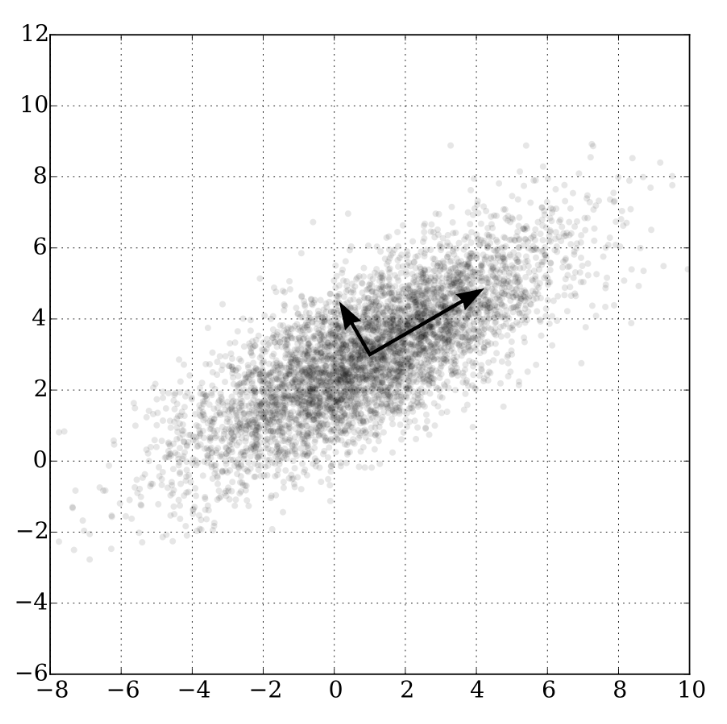
\includegraphics[width=0.8\linewidth]{fig/pca.png}
    \caption{Principal Component Analysis ของข้อมูลที่มีการกระจายตัวแบบเกาส์เซียนหลายตัวแปร (Multivariate Gaussian
    Distribution) เวกเตอร์ที่แสดงนั้นเป็น Eigenvector ของ Covariance Matrix ที่มีการปรับขนาด (Scaled) โดยใช้ค่ายกกำลังสองของ 
    Eigenvalue และมีการปรับตำแหน่งโดยใช้ค่าเฉลี่ย}
    \label{fig:pca}
\end{figure}

การวิเคราะห์องค์ประกอบหลักหรือ Principal Component Analysis (PCA) เป็นวิธีทางสถิติที่ถูกเอามาใช้เพื่อรับมือกับข้อมูลที่มี
จำวนหลายมิติหรือมีหลายตัวแปร โดย PCA สามารถหาความสัมพันธ์ของตัวแปรเหล่านั้นโดยทำการลดขนาดของมิติโดยสร้างชุดข้อมูลใหม่ที่อาศัย
แกนอ้างอิงจากชุดข้อมูลเดิม ซึ่งจำนวนมิติที่ถูกลดลงนั้นก็มีจำนวนมิติเพียง 2 หรือ 3 มิติเท่านั้น ซึ่งทำให้ง่ายต่อการตีความและวิเคราะห์ข้อมูล เช่น
การจัดกลุ่มชุดข้อมูลโดยจำแนกตาม Feature ซึ่ง Feature แต่ละคู่จะมีคุณสมบัติ Orthogonality หรือตั้งฉากกันนั่นเอง ทำให้เราสามารถแสดง
ผลลัพธ์ของ PCA ออกมาได้ในปริภูมิทั่วไป

%--------------------------
\section{การเข้ารหัสแบบอัตโนมัติ}
\idxboth{การเข้ารหัสแบบอัตโนมัติ}{Autoencoder}
%--------------------------

การเข้ารหัสแบบอัตโนมัติหรือ Autoencoder

\begin{center}
\begin{tikzpicture}[x=2.1cm,y=1.2cm]
    % \large
    \message{^^JNeural network without arrows}
    \readlist\Nnod{6,5,4,3,4,5,6} % array of number of nodes per layer
    
    % TRAPEZIA
    \node[above,align=center,myorange!60!black] at (3,2.4) {Encoder};
    \node[above,align=center,myblue!60!black] at (5,2.4) {Decoder};
    \draw[myorange!40,fill=myorange,fill opacity=0.02,rounded corners=2]
    (1.6,-2.7) --++ (0,5.4) --++ (2.8,-1.2) --++ (0,-3) -- cycle;
    \draw[myblue!40,fill=myblue,fill opacity=0.02,rounded corners=2]
    (6.4,-2.7) --++ (0,5.4) --++ (-2.8,-1.2) --++ (0,-3) -- cycle;
    
    \message{^^J  Layer}
    \foreachitem \N \in \Nnod{ % loop over layers
    \def\lay{\Ncnt} % alias of index of current layer
    \pgfmathsetmacro\prev{int(\Ncnt-1)} % number of previous layer
    \message{\lay,}
    \foreach \i [evaluate={\y=\N/2-\i+0.5; \x=\lay; \n=\nstyle;}] in {1,...,\N}{ % loop over nodes
    
    % NODES
    \node[node \n,outer sep=0.6] (N\lay-\i) at (\x,\y) {};
    
    % CONNECTIONS
    \ifnum\lay>1 % connect to previous layer
    \foreach \j in {1,...,\Nnod[\prev]}{ % loop over nodes in previous layer
    \draw[connect,white,line width=1.2] (N\prev-\j) -- (N\lay-\i);
    \draw[connect] (N\prev-\j) -- (N\lay-\i);
    %\draw[connect] (N\prev-\j.0) -- (N\lay-\i.180); % connect to left
    }
    \fi % else: nothing to connect first layer
    
    }
    }
    
    % LABELS
    \node[above=2,align=center,mygreen!60!black] at (N1-1.90) {Input};
    \node[above=2,align=center,myred!60!black] at (N\Nnodlen-1.90) {Output};
    
\end{tikzpicture}
\end{center}

ตัวเข้ารหัสแบบอัตโนมัติหรือ Autoencoder (AE) เป็นอัลกอริทึม Unsupervised Learning แบบหนึ่งที่สร้างโมเดล ANN โดยมีรูปแบบของ 
Network ที่เฉพาะตัวนั่นก็คือจะทำการลดหรือบีบอัดข้อมูล (Encoder) และทำการถอดรหัส (Decoder) ออกมาเป็นข้อมูลเดิม\cite{ballard1987} 
ตัวโมเดล AE มีความพิเศษคือจะมีลักษณะของความสมมาตร นอกจากนี้ยังมีความแตกต่างจาก PCA นั่นก็คือสามารถบีบอัดหรือลดจำนวนมิติของข้อมูล%
แบบไม่เป็นเส้นตรงได้ (Nonlinear) ได้ด้วยการใช้ Nonlinear Activation Function 

%--------------------------
\section{การแบ่งกลุ่มข้อมูลแบบเคมีน}
\idxen{K-means Clustering}
%--------------------------

การแบ่งกลุ่มข้อมูลแบบเคมีนหรือ K-means Clustering

\begin{figure}[H]
    \centering
    \subfloat[\label{fig:k_mean_step1}]{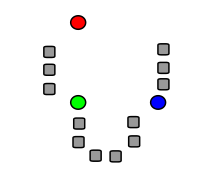
\includegraphics[width=0.4\linewidth]{fig/k-mean-step1.png}}
    \subfloat[\label{fig:k_mean_step2}]{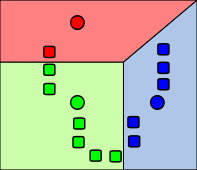
\includegraphics[width=0.4\linewidth]{fig/k-mean-step2.png}}
    \\
    \subfloat[\label{fig:k_mean_step3}]{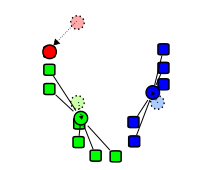
\includegraphics[width=0.4\linewidth]{fig/k-mean-step3.png}}
    \subfloat[\label{fig:k_mean_step4}]{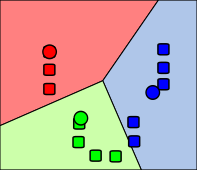
\includegraphics[width=0.4\linewidth]{fig/k-mean-step4.png}}
    \caption{ขั้นตอนการทำ K-mean Clustering (เครดิตภาพ: \url{https://en.wikipedia.org/wiki/K-means_clustering})}
    \label{fig:k_mean}
\end{figure}
 